\graphicspath{{./MKL/img/}}
\chapter{Multiple Kernels}
\label{C:MKL}
In this chapter we introduce a framework for two sample testing based
on heterogeneous data based on multiple kernel learning (MKL).

\section{Introduction}
Introduction to MKL, theory of MKL, and optimization problems/tuning
parameters.  

\section{Simulations}
\subsection{Vectorial Data Mixture Distribution}
Let's look at mixtures of MVN.  Let
\begin{align*}
  \Sigma_1 &=
  \begin{bmatrix}
    1^2 & 0   \\
    0   & 1^2 \\
  \end{bmatrix} \\
  \Sigma_2 &=
  \begin{bmatrix}
    10^2 & 0   \\
    0    & 10^2 \\
  \end{bmatrix} \\
  \mu_1(\delta_1) &= [\delta_1, 0]^T \\
  \mu_2(\delta_2) &= [\delta_2, 100]^T. \\
\end{align*}

Let $d_1$ be a mixture distribution of $\mathcal{N}_2([0, 0]^T, \Sigma_1)$ with
probability $p$ and $\mathcal{N}_2([0, 100]^T, \Sigma_2)$ with
probability $1-p$.  Let $d_2$ be a mixture distribution of
$\mathcal{N}_2([1, 0]^T, \Sigma_1)$ with probability $p$ and
$\mathcal{N}_2([10, 100]^T, \Sigma_2)$ with probability $1-p$.  Note
that $\delta_1 = 1$ and $\delta_2 = 10$ were chosen to be one standard
deviation away (on the x-axis, see $(\Sigma_1)_{1,1}$ and
$(\Sigma_2)_{1,1}$).  In all the simulations, we draw $n = 50$ samples
from each mixture distribution, $d_1$ and $d_2$.  We take the mixture
probability $p = .5$ unless otherwise specified.

Here is a plot of the 95\% confidence ellipses of the mixture distributions:
\begin{figure}[!ht]
  \centering
  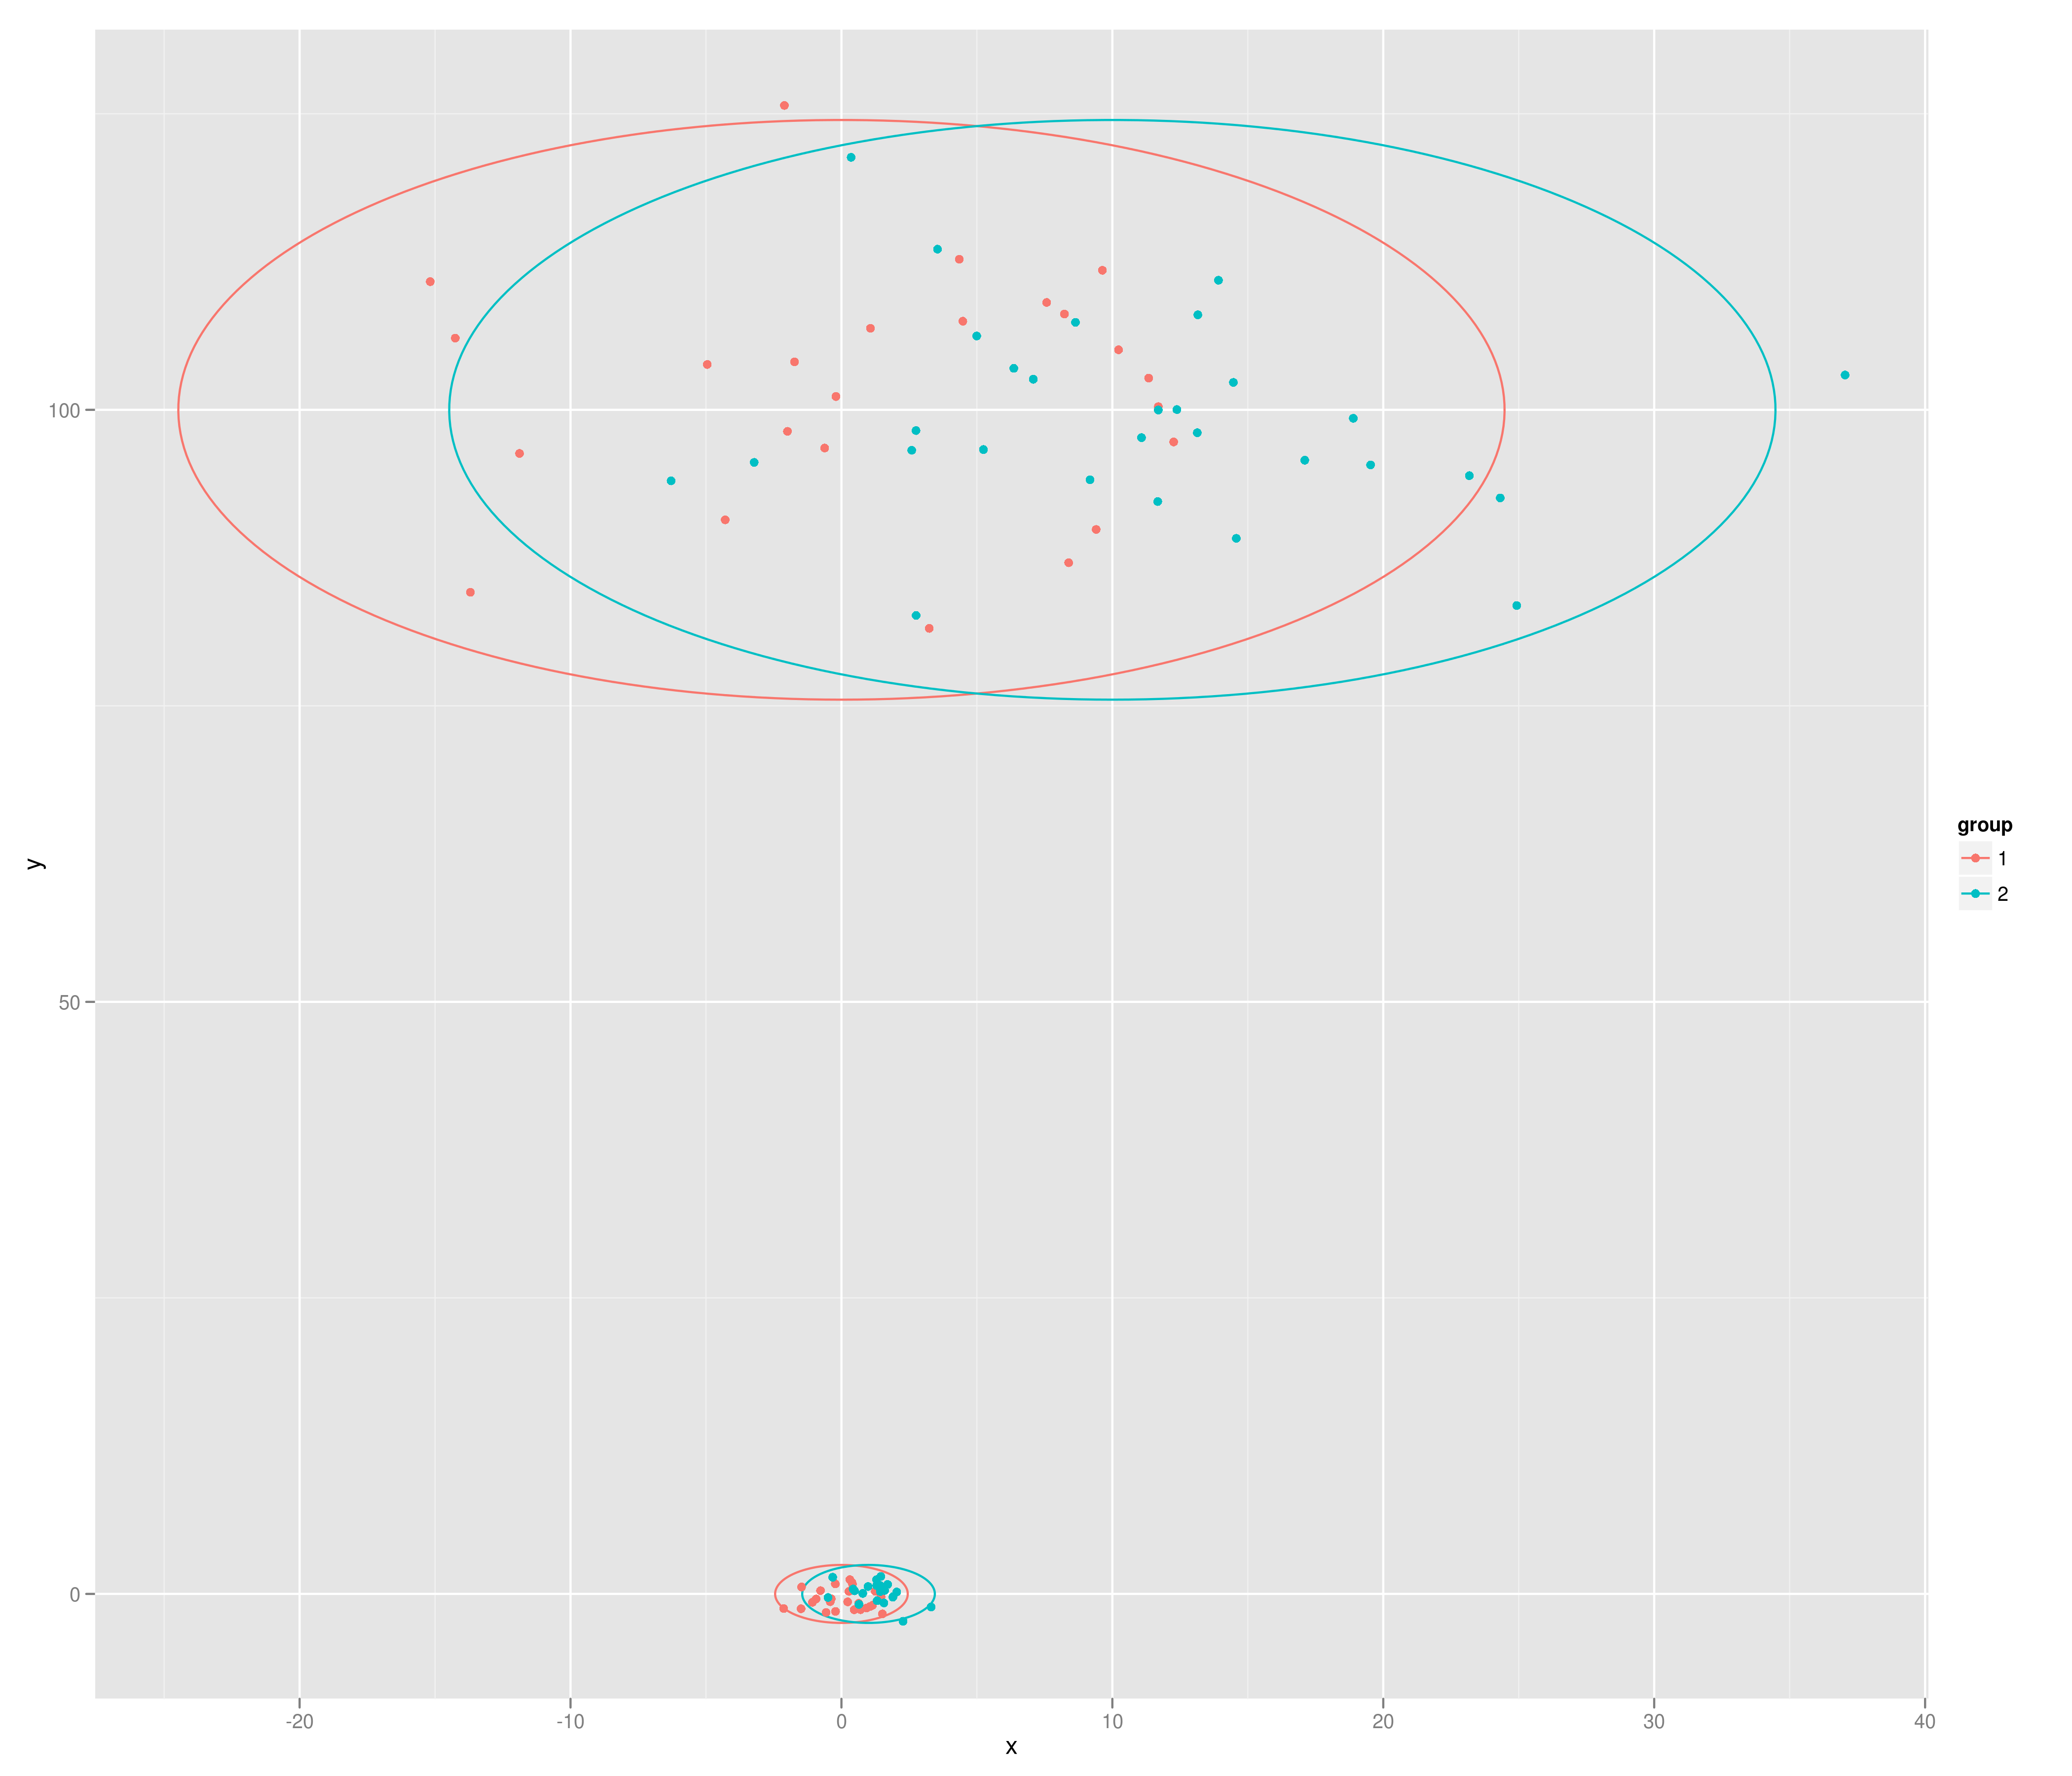
\includegraphics[scale=.3]{p5.png}  
\end{figure}

Here we plot the average power and bootstrap 95\% confidence intervals
(100 simulations) for each RBF kernel individually and MKL on all of
them, faceted on the mixture probability.  So for $p = 0$, we have all
the weight on $\mathcal{N}_2(\mu_2, \Sigma_2)$, and for $p = 1$, we
have all the weight on $\mathcal{N}_2(\mu_1, \Sigma_1)$.  Since the
latter is on a smaller scale, we expect the smaller width RBF kernels
to do better.  We take $C = 1$, and the widths to be from the middle
run of the last section:
\begin{figure}[!ht]
  \centering
  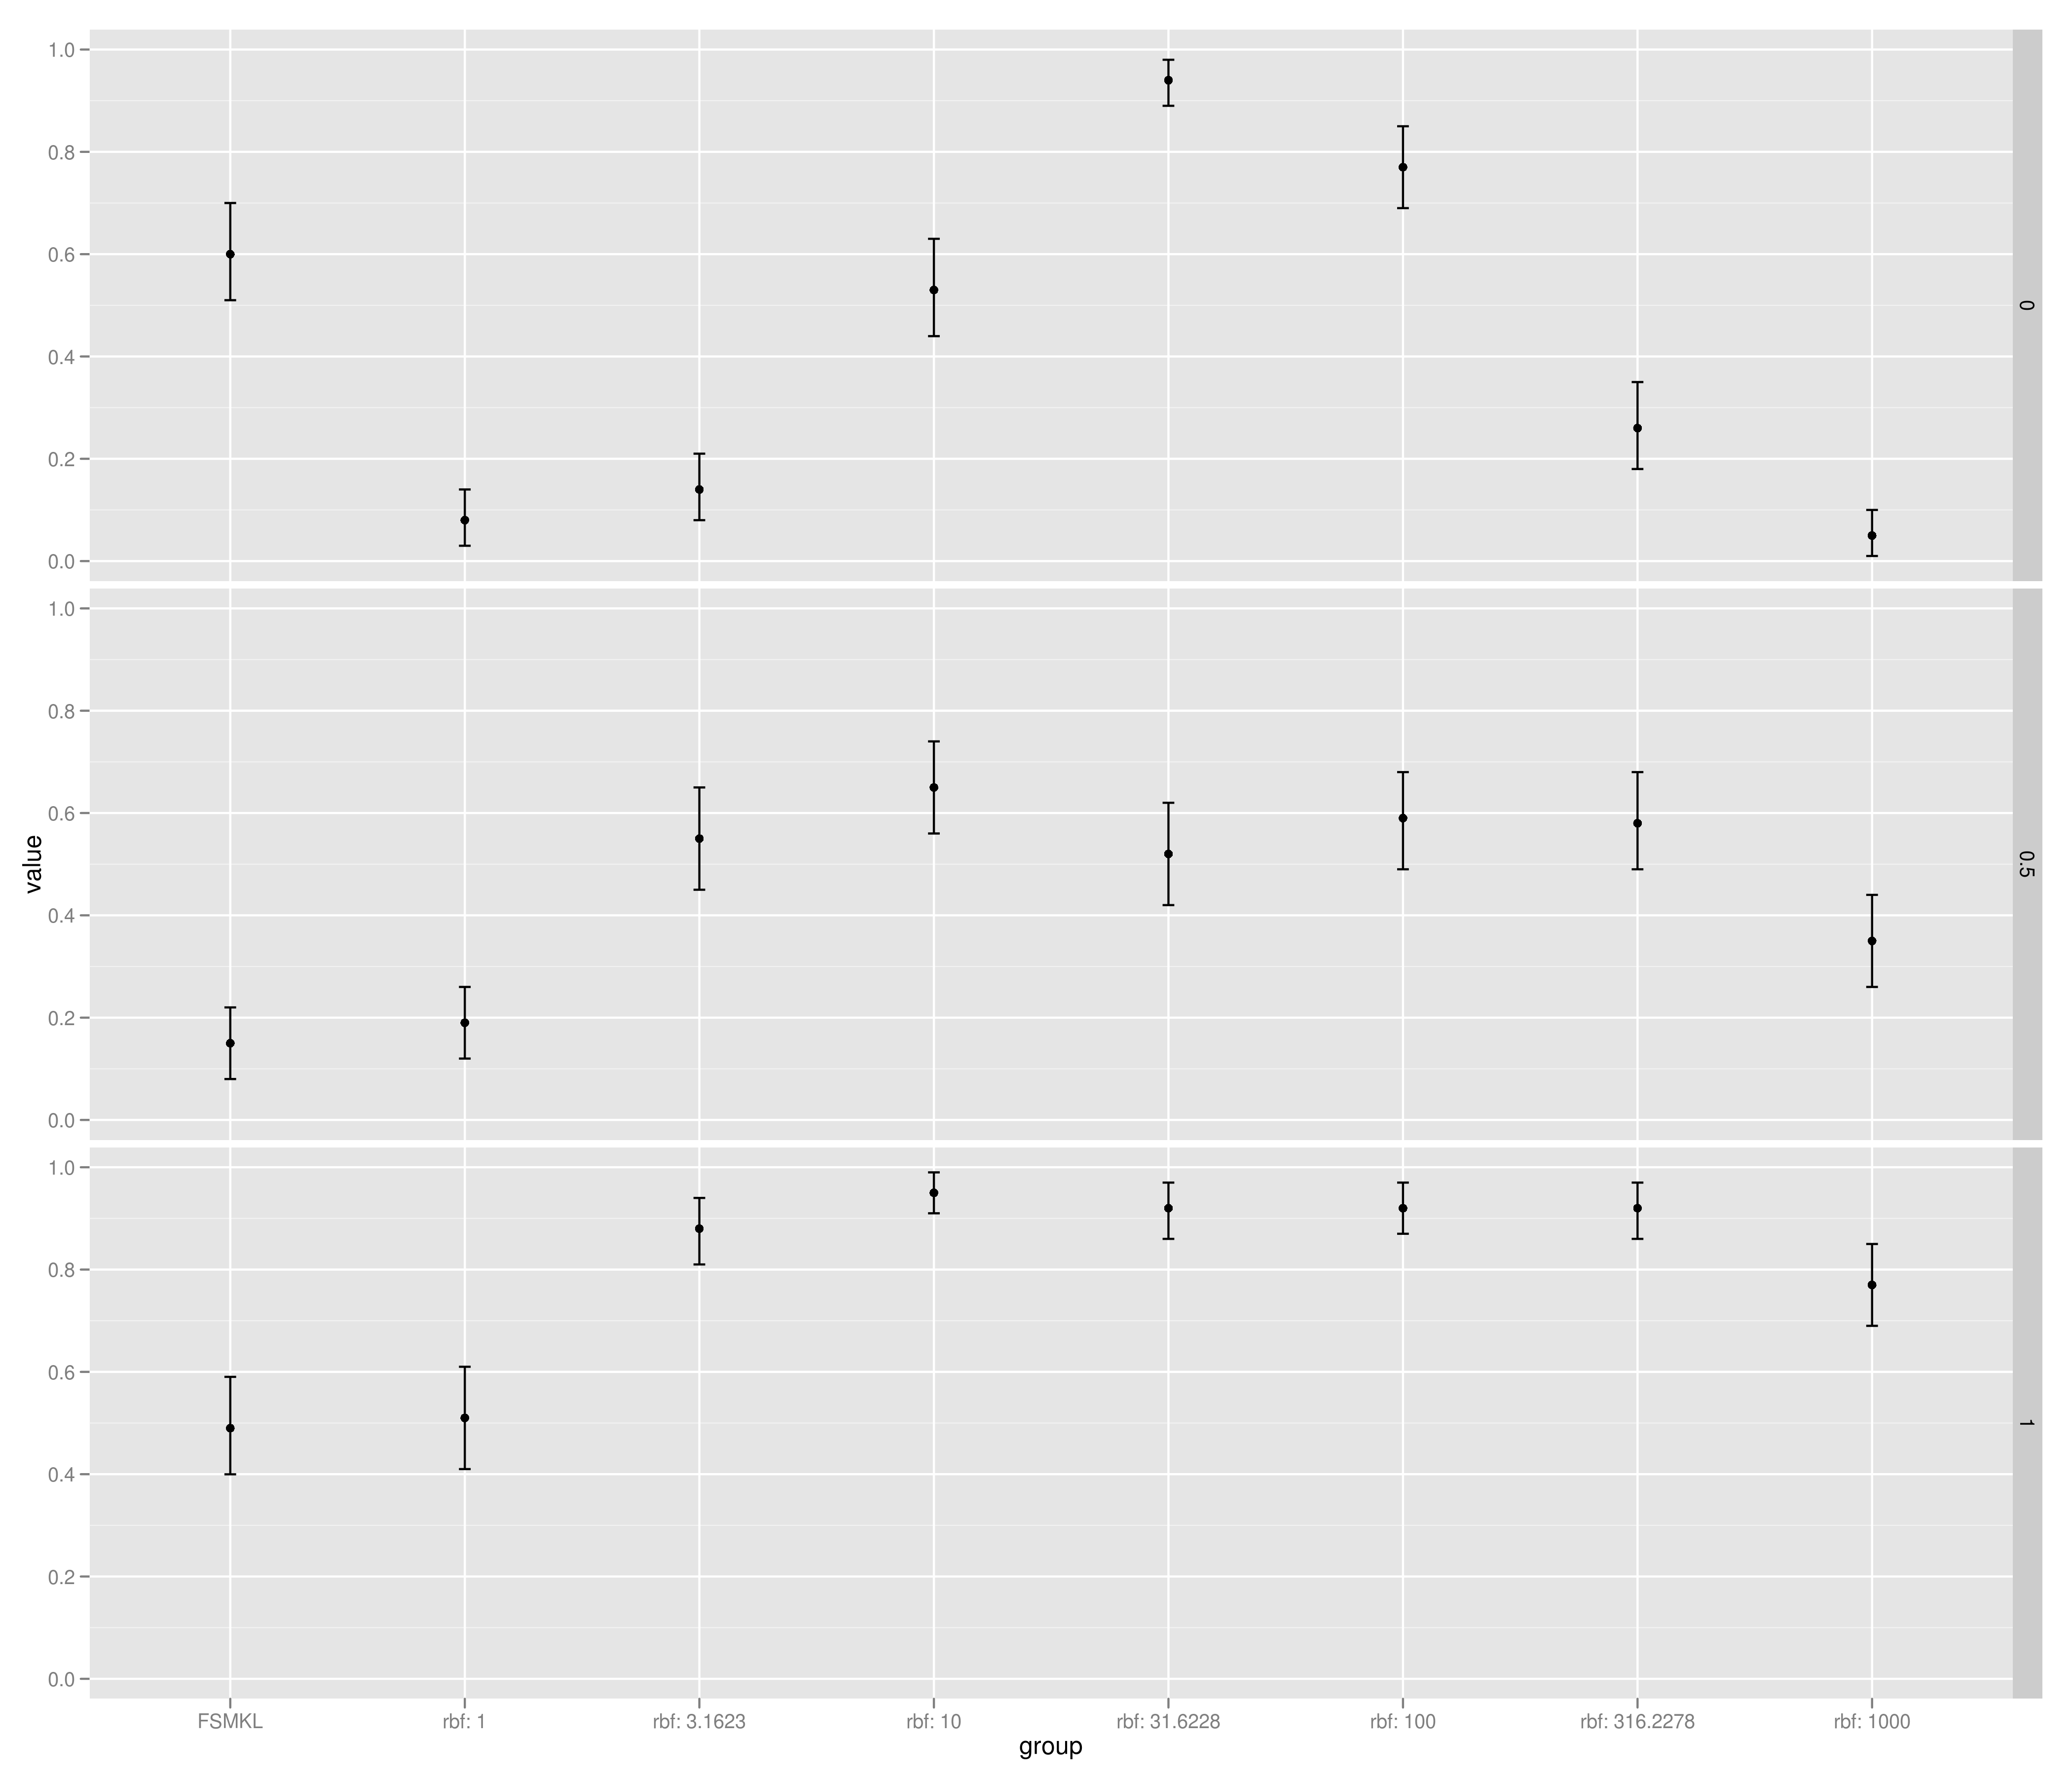
\includegraphics[scale=.3]{p4-2.png}
\end{figure}
The smaller distribution ($p=1$) has higher power for smaller kernels,
but the MKL power is about the same as compared with the $p=0$ case.
Both outperform the mixed setting.




Example with heterogeneous data (vectorial + string).

\section{Wine Example}
TODO
